\documentclass[a4paper,12pt,oneside,openany,autodetect-engine,dvipdfmx,platex]{jsreport}
\usepackage{latexsym}
\usepackage{booktabs}
\usepackage{color}
\usepackage{colortbl}
\usepackage{graphicx}
\usepackage{amsmath}
\usepackage{bm}
\usepackage{multirow}
\usepackage{hyperref}
\usepackage{pxjahyper}
\newcommand{\ChangeHeaderRule}{%
     \let\subsubsection\subsection
     \let\subsection\section
     \let\section\chapter
}

%%%%%%%%%%%%%%%%%%%%%%%%%%%%
% 表紙
%%%%%%%%%%%%%%%%%%%%%%%%%%%%
\begin{document}

\begin{titlepage}
\begin{flushright}
%{\large
指導教員(主査):山本祐輔 講師\\
副査:XXX 教授
%}
\end{flushright}
\begin{center}
\vspace*{80pt}
{\large 2019年度 静岡大学情報学部 卒業論文}\\

\vspace*{40pt}
{\huge XXXに関する研究}\\
\vspace{10pt}
{\Large --- サブタイトル ---}\\
\vfill
{静岡大学 情報学部 行動情報学科 所属}\\
{学籍番号 XXXXX}\\
\vspace{20pt}
{静岡 花子}\\
\vspace{20pt}
{\today}\\
\end{center}
\vfill
\end{titlepage}


%%%%%%%%%%%%%%%%%%%%%%%%%%%%
% アブストラクト(300字程度)
%%%%%%%%%%%%%%%%%%%%%%%%%%%%
\begin{abstract}
\input{section/abstract}
\end{abstract}

%%%%%%%%%%%%%%%%%%%%%%%%%%%%
% 目次
%%%%%%%%%%%%%%%%%%%%%%%%%%%%

\tableofcontents

\newpage
\listoffigures
\listoftables


%%%%%%%%%%%%%%%%%%%%%%%%%%%%
% 本文
%%%%%%%%%%%%%%%%%%%%%%%%%%%%
\ChangeHeaderRule

% 0章:LateXの使い方
\input{section/how-to-use-latex}

% 1章:はじめに
\section{はじめに}\label{sec:introduction}
この章は研究の導入を語る章です.
以下は画像の挿入例です(\ref{fig:example}).
参考文献も引用できます\cite{Yamamoto2018}.

\begin{figure}
  \centering
  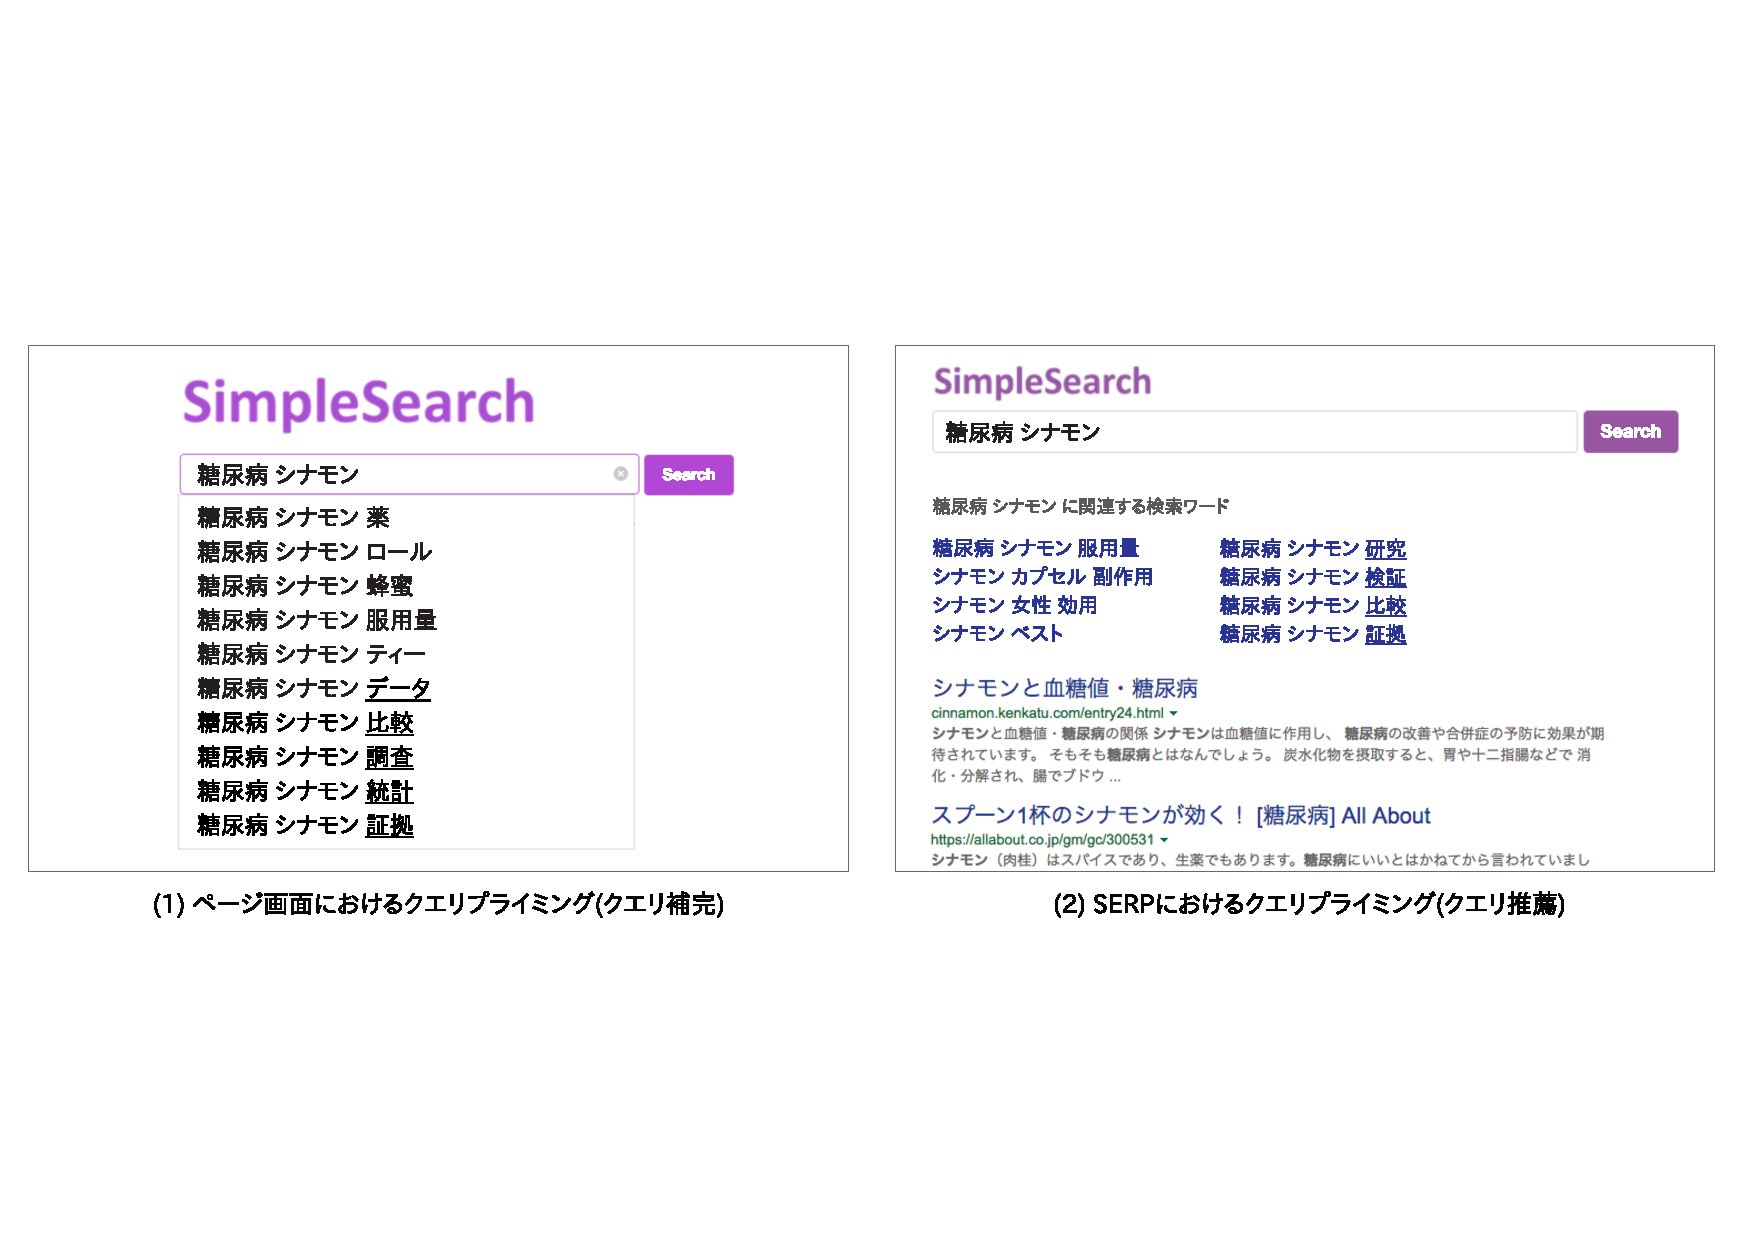
\includegraphics[width=15cm]{figure/example.pdf}
  \caption{画像のサンプル}
  \label{fig:example}
\end{figure}


% 2章:関連研究
\section{関連研究}\label{sec:related-works}
これは関連研究の章です.


% 3章:提案事項
\section{提案内容}\label{sec:approach}
この章は提案手法について記す章です.


% 4章:評価実験
\section{実験}\label{sec:experiment}
この章は実験方法に関する考察を記す章です.


% 5章:結果
\section{結果}\label{sec:results}
これは実験の結果を記す章です.


% 6章:考察
\section{考察}\label{sec:introduction}
この章は実験結果に関する考察を記す章です.


% 7章:おわりに
\section{おわりに}\label{sec:conclusion}
この章は論文のまとめを記す章です.



\vspace{2em}

% 参考文献リスト
\markboth{参考文献}{参考文献}
\begin{thebibliography}{99}
\bibitem{Yamamoto2018}
Yamamoto, Y. and Yamamoto, T. (2018) ``Query Priming for Promoting Critical Thinking in Web Search'',\textit{Proceedings of the 3rd ACM SIGIR Conference on Human Information Interaction and Retrieval (CHIIR 2018)},pp.12-21, ACM.
\end{thebibliography}

% 謝辞
\section*{謝辞}
これは謝辞を記す箇所です.

\begin{flushright}
2020年3月 XXX XXX
\end{flushright}

\end{document}
